

\actTitle{Worksheet 4.3}



\noindent \textbf{Instructions:}  Work together in groups of  3 or 4 to complete the following problems.\\


\begin{enumerate}

\item Find the exact values of the six trigonometric functions of $\theta$ and $\alpha$
\begin{enumerate}
\item Use the following triangle.\\

\newcommand{\trigTriangle}[5]{%
	\begin{tikzpicture}[scale=2.5]
	\draw (0,0) -- (2,0) -- (2,1) -- (0,0);
	\draw (1.9,0) -- (1.9,0.1) -- (2,0.1);
	\draw (0.3,0) arc(0:40:0.2);
	\draw (0.5,0.1) node { #1 };
	\draw (1.8,0.7) node { #2 };
	\draw (1,-0.1) node { #3 };
	\draw (1,0.6) node { #4 };
	\draw (2,0.8) arc(270:210:0.2);
	\draw (2.1,0.5) node { #5 };
	\end{tikzpicture}
}

	\trigTriangle{$\theta$}{$\alpha$}{8}{10}{6}

\vfill
\item Use the following triangle.\\
\trigTriangle{$\theta$}{$\alpha$}{15}{ }{8}
\vfill
\end{enumerate}

\newpage 

\item Use the isosceles right triangle and the 30/60/90 triangle to complete the table.

\begin{table}[h]
\begin{tabular}{|l|l|l|l|l|l|l|}
\hline
\textbf{$\theta$}        & \textbf{$\sin(\theta)$} & \textbf{$\cos(\theta)$} & \textbf{$\tan(\theta)$} & \textbf{$\csc(\theta)$} & \textbf{$\sec(\theta)$} & \textbf{$\cot(\theta)$} \\ \hline
30$^\circ=\frac{\pi}{6}$ &                         &                         &                         &                         &                         &                         \\ \hline
45$^\circ=\frac{\pi}{4}$ &                         &                         &                         &                         &                         &                         \\ \hline
60$^\circ=\frac{\pi}{3}$ &                         &                         &                         &                         &                         &                         \\ \hline
\end{tabular}
\end{table}

\begin{tikzpicture}[y=5cm, x=5cm,font=\sffamily]
  \draw[thick,black] (0,0) -- (1,0) -- (1,1) -- cycle;
  \draw[very thin,black] (0.8,0.0) -- (0.8,0.2) -- (1,0.2);
  \draw[thin,black] (0.2,0) arc (0:45:0.2);
  \node[black,anchor=north] at (0.5,0) {1};
  \node[black,anchor=west] at (1,0.5) {1};
  \node[black,anchor=south east] at (45:0.7) {$\sqrt{2}$};
  \node[black,anchor=south west] at (12.5:0.2) {$45^\circ$};

  \draw[thin,black] (45:1.25) arc (225:270:0.17);
  \node[black,anchor=west,xshift={8pt}] at (45:1.1) {$45^\circ$};
\end{tikzpicture}

\begin{tikzpicture}[y=5cm, x=5cm,font=\sffamily]
  \draw[thick,black] (0,0) -- (1,0) -- (60:2) -- cycle;
  \draw[thick,black,dashed] (1,0) -- (2,0) -- (60:2);
  \draw[very thin,black] (0.8,0.0) -- (0.8,0.2) -- (1,0.2);
  \draw[thin,black] (0.2,0) arc (0:60:0.2);
  \node[black,anchor=north] at (0.5,0) {1};
  \node[black,anchor=west] at (1,0.8) {$\sqrt{3}$};
  \node[black,anchor=south east] at (60:1) {$2$};
  \node[black,anchor=south west] at (12.5:0.2) {$60^\circ$};
  \draw[thin,black] (60:1.8) arc (240:270:0.2);
  \node[black,anchor=west] at (60:1.65) {$30^\circ$};
\end{tikzpicture}

\vfill

%\item
%\begin{enumerate}
%\item Evaluate $\sin(60^\circ)$.\\[0.2in]
%\item Evaluate $\sin(30^\circ)+\sin(30^\circ)$.\\[0.2in]
%\item Are the values in parts $(a)$ and $(b)$ the same?
%\end{enumerate}

\newpage




\item For each problem below determine the values of the missing quantities. All angles are in radians, and your answers for angles should be in radians. (The triangles are not drawn to scale.)
\begin{enumerate}
\item \newcommand{\trigTriangle}[5]{%
	\begin{tikzpicture}[scale=2.5]
	\draw (0,0) -- (2,0) -- (2,1) -- (0,0);
	\draw (1.9,0) -- (1.9,0.1) -- (2,0.1);
	\draw (0.3,0) arc(0:40:0.2);
	\draw (0.5,0.1) node { #1 };
	\draw (1.8,0.7) node { #2 };
	\draw (1,-0.1) node { #3 };
	\draw (1,0.6) node { #4 };
	\draw (2,0.8) arc(270:210:0.2);
	\draw (2.1,0.5) node { #5 };
	\end{tikzpicture}
}



\trigTriangle{$\pi/4$}{$\alpha$}{a}{4}{b}
	
	\framebox[0.3\textwidth][l]{
		\begin{tabular}{lc}
			$a$ & $=$ \\ [15pt]
			$b$ & $=$ \\ [15pt]
			$\alpha$ & $=$ \\
		\end{tabular}
	}
	\vfill

\item \trigTriangle{$\pi/6$}{$\psi$}{2}{h}{b}
	
	\framebox[0.3\textwidth][l]{
		\begin{tabular}{lc}
			$b$ & $=$ \\ [15pt]
			$h$ & $=$ \\ [15pt]
			$\psi$ & $=$ \\
		\end{tabular}
	}
	\vfill

\end{enumerate}
\newpage

\item If a 15 ft ladder is leaning against a wall at an angle of $62^\circ$ with the ground, how high up the will will the ladder reach?  Round to the nearest tenth of a foot.\vfill

\item A 30 ft boat ramp makes a $7^\circ$ angle with the water.  What is the height of the ramp above the water at the ramp's highest point?  Round to the nearest tenth of a foot.\vfill

\item At a tree farm, palm trees are harvested once they reach a height of 20 feet.  Suppose a farm worker determine's that the distance along the ground from her position to the base of a palm tree is 22 feet.  She then uses an instrument called a clinometer held at her eye level of 6 feet to measure the angle of elevation tot he top of the tree as $30.2^\circ$.  Is the tree tall enough to harvest?\vfill
%\newpage
%
%\item The following is the unit circle.  \\
%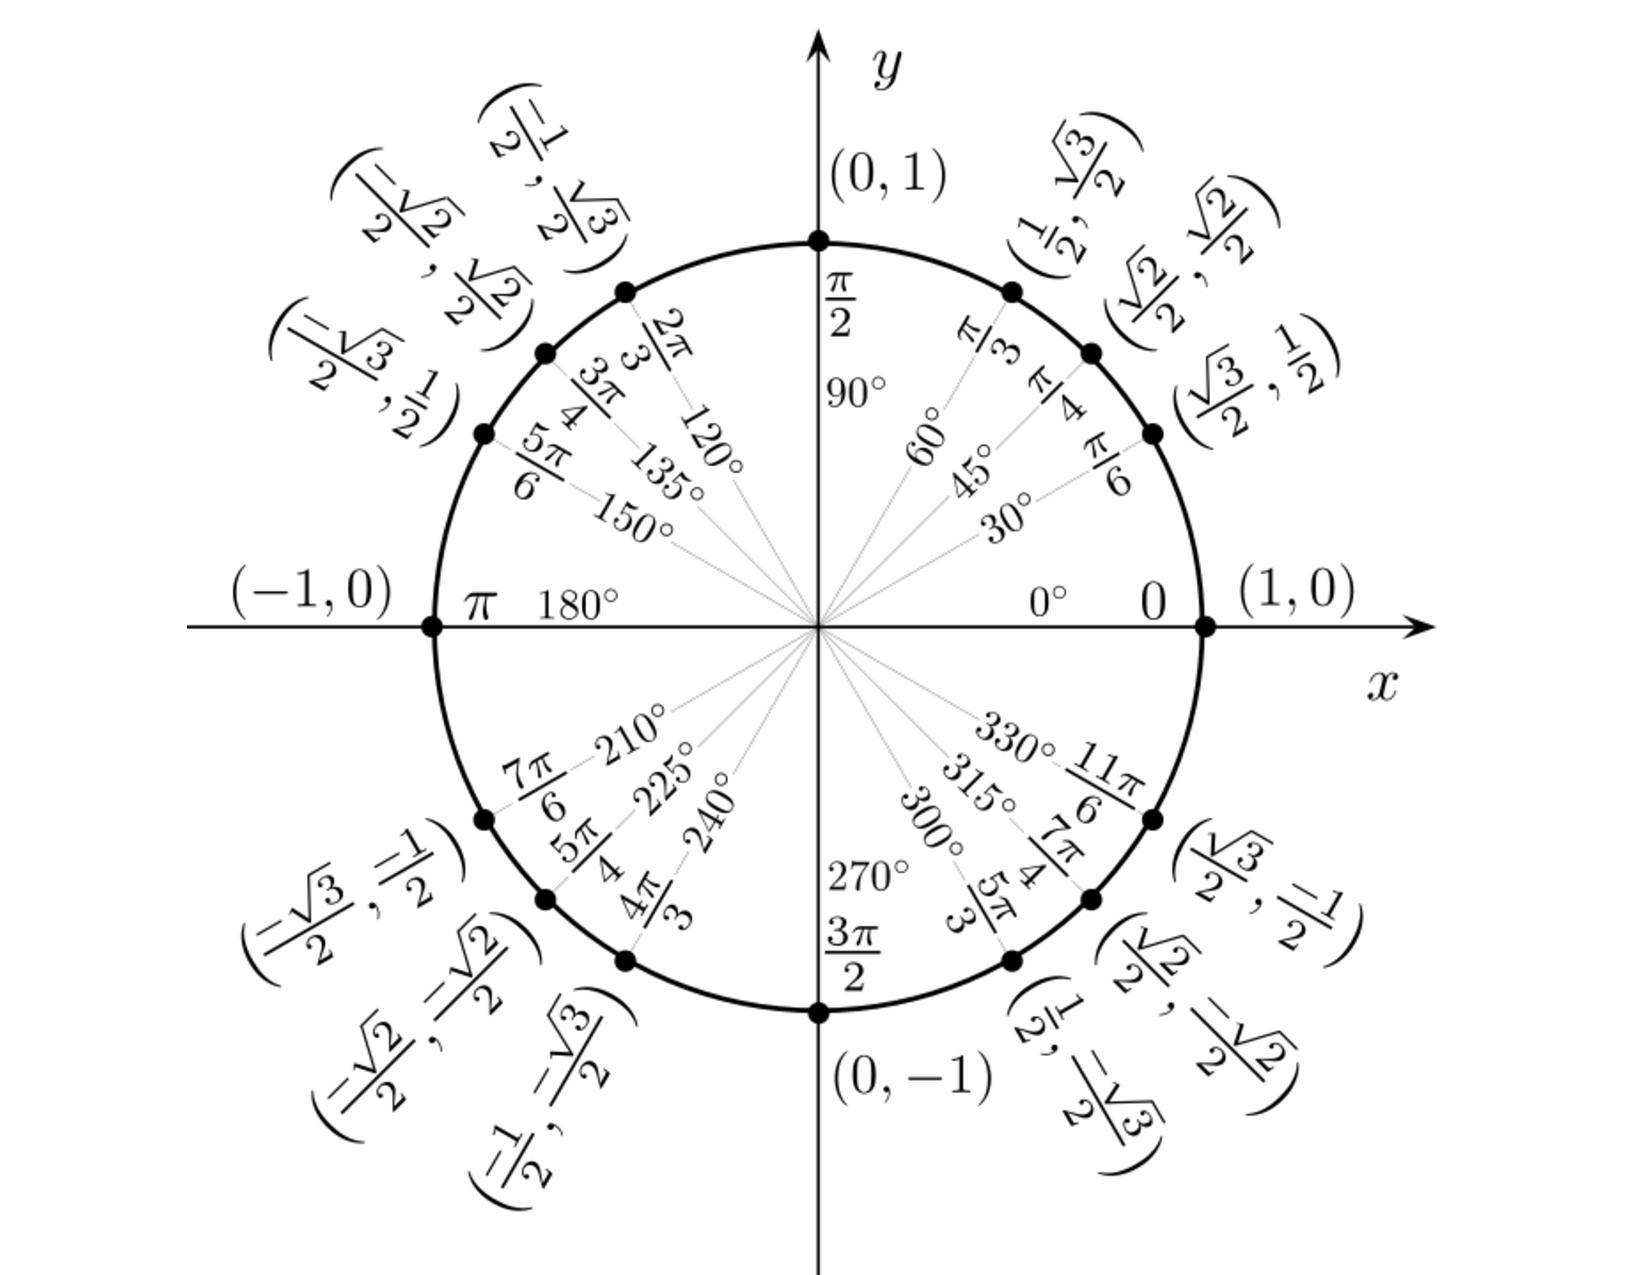
\includegraphics[scale=.7]{unit_circle}
%\begin{enumerate}
%\item Use the first quadrant to verify your answers in the table in Question 2.\\
%\item Determine the radius of this circle.\\
%
%\end{enumerate}
\end{enumerate}

